\documentclass[tikz,border=5pt]{standalone}
\usepackage{amsmath,amssymb}
\usetikzlibrary{arrows.meta,positioning,calc,shapes.geometric}
\begin{document}
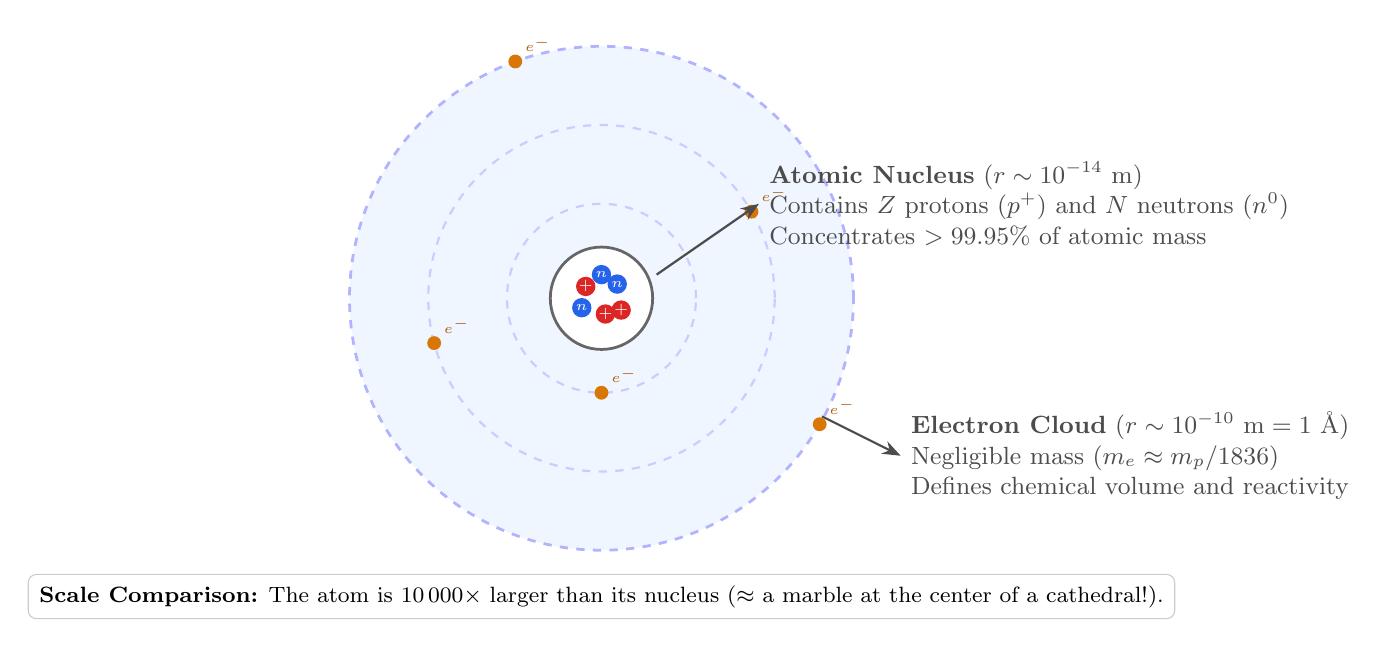
\begin{tikzpicture}[>=Stealth, font=\sffamily]
  \definecolor{protonred}{HTML}{DC2626}
  \definecolor{neutronblue}{HTML}{2563EB}
  \definecolor{electronyellow}{HTML}{D97706}
  \definecolor{cloudcolor}{HTML}{EFF6FF}

  % Electron cloud
  \fill[cloudcolor] (0,0) circle (3.2cm);
  \draw[blue!30, dashed, line width=1pt] (0,0) circle (3.2cm);
  \draw[blue!20, dashed, line width=0.8pt] (0,0) circle (2.2cm);
  \draw[blue!20, dashed, line width=0.8pt] (0,0) circle (1.2cm);

  % Orbiting electrons
  \foreach \angle/\rad in {30/2.2, 110/3.2, 195/2.2, 270/1.2, 330/3.2} {
    \fill[electronyellow] (\angle:\rad) circle (2.5pt);
    \node[anchor=south west, font=\tiny\bfseries, text=electronyellow!80!black] at (\angle:\rad) {$e^-$};
  }

  % Central nucleus
  \draw[black!60, fill=white, line width=1pt] (0,0) circle (0.65cm);
  % Nucleons
  \fill[protonred] (-0.2,0.15) circle (3.5pt) node[white, font=\tiny\bfseries] {$+$};
  \fill[neutronblue] (0.2,0.18) circle (3.5pt) node[white, font=\tiny\bfseries] {$n$};
  \fill[protonred] (0.05,-0.2) circle (3.5pt) node[white, font=\tiny\bfseries] {$+$};
  \fill[neutronblue] (-0.25,-0.12) circle (3.5pt) node[white, font=\tiny\bfseries] {$n$};
  \fill[protonred] (0.25,-0.15) circle (3.5pt) node[white, font=\tiny\bfseries] {$+$};
  \fill[neutronblue] (0.0,0.3) circle (3.5pt) node[white, font=\tiny\bfseries] {$n$};

  % Annotations
  \draw[->, thick, black!70] (0.7,0.3) -- (2.0,1.2) node[right, align=left, font=\small] {
    \textbf{Atomic Nucleus} ($r \sim 10^{-14}\ \mathrm{m}$)\\
    Contains $Z$ protons ($p^+$) and $N$ neutrons ($n^0$)\\
    Concentrates $> 99.95\%$ of atomic mass
  };

  \draw[->, thick, black!70] (2.8,-1.5) -- (3.8,-2.0) node[right, align=left, font=\small] {
    \textbf{Electron Cloud} ($r \sim 10^{-10}\ \mathrm{m} = 1\ \text{\AA}$)\\
    Negligible mass ($m_e \approx m_p / 1836$)\\
    Defines chemical volume and reactivity
  };

  % Scale banner
  \node[anchor=north, draw=gray!40, fill=white, rounded corners=3pt, inner sep=4pt, font=\footnotesize] at (0,-3.5) {
    \textbf{Scale Comparison:} The atom is $10\,000\times$ larger than its nucleus ($\approx$ a marble at the center of a cathedral!).
  };
\end{tikzpicture}
\end{document}
